\documentclass[11pt,a4paper]{book}
\usepackage[utf8]{inputenc}
\usepackage[T1]{fontenc}
\usepackage[left=2cm,right=2cm,top=2cm,bottom=2cm]{geometry}
\usepackage[spanish, activeacute]{babel}
\usepackage{amsmath}
\usepackage{amssymb,amsfonts,textcomp}
\usepackage{color}
\usepackage{array}
\usepackage{hhline}
\usepackage{hyperref}
\usepackage{graphicx}
\hypersetup{ colorlinks=true, linkcolor=black, citecolor=black, filecolor=black, urlcolor=blue, pdftitle=Romulo y Remo, pdfauthor=alberto, pdfsubject=, pdfkeywords=}
% Outline numbering

% Page layout (geometry)

% Footnote rule
\setlength{\skip\footins}{0.119cm}
\renewcommand\footnoterule{\vspace*{-0.018cm}\setlength\leftskip{0pt}\setlength\rightskip{0pt plus 1fil}\noindent\textcolor{black}{\rule{0.25\columnwidth}{0.018cm}}\vspace*{0.101cm}}
% Pages styles


\title{\Huge{\textbf{Romulo y Remo}}
\begin{figure}[hbtp]
		\centering
		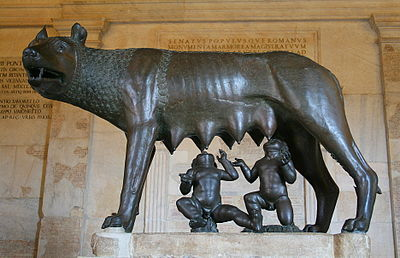
\includegraphics[width= 80mm ]{E:/workspace/TFG/TFG/WebContent/imagenes/1435502934359.JPG}
	\end{figure}}
\author{alberto}
\begin{document}
\maketitle

\tableofcontents


			\chapter{La leyenda}
												Genealogía[editar]
	\bigskip
							Cuenta la leyenda antiquísima de los helenos que Eneas, príncipe de Dardania, escapó de la destrucción de Troya cargando a su padre, Anquises, sobre sus hombros y a su hijo Ascanio, aunque perdió en la fuga a su esposa, Creúsa, hija del rey Príamo. Esto sucedió en torno a 1184 a. C. según el erudito antiguo Eratóstenes (276-194 a. C.), tras diez años de conflicto.3 Tres décadas después de periplos Ascanio fundó la urbe de Alba Longa de la que fue su primer rey. Cuatro siglos después vendría el tiempo del rey Numitor.4
	\bigskip
							
	\bigskip
							Infancia y juventud[editar]
	\bigskip
							Numitor fue destituido entonces por su hermano Amulio, que acabó con todos los hijos varones de éste y convirtió a su única hija, Rea Silvia, en una virgen vestal para que así, al tener un voto de castidad, no tuviera descendientes,5 pero el dios de la guerra, Marte, se enamoró de la bella muchacha y la sedujo; de su unión se engendraron dos gemelos, Rómulo y Remo.6 Varrón llegó incluso a calcular las fechas exactas de cuando fueron concebidos (24 de junio de 772 a. C.) y de su nacimiento (24 de marzo de 771 a. C.).7
	\bigskip
							
	\bigskip
							Amulio, temeroso de tener en el futuro dos posibles rivales, ordenó su asesinato pero el hombre encargado del infanticidio no pudo y los abandonó a su suerte en el río Tíber.8 La corriente llevó la cesta donde estaban a un pantano llamado Velabrum, en un lugar entre las colinas Palatino y Capitolio llamado Cermalus.9 Ahí fueron cuidados y alimentados por una loba llamada Luperca y un pájaro carpintero, los animales sagrados de Marte.10 Poco después los encontró el pastor Faustolo, que era porquerizo de Amulio, y decidió criar en secreto a los niños con su esposa Acca Larenzia.11 Sólo una vez que crecieron se les reveló su verdadera identidad y éstos decidieron tomar justicia. Mataron a Amulio y liberaron de su encierro a su abuelo que fue repuesto en su trono.12
	\bigskip
							
	\bigskip
							Fundación de Roma[editar]
	\bigskip
							Rómulo y Remo partieron de Alba Longa, pues querían gobernar, pero no derrocar a su abuelo. Marcharon al lugar donde el pastor los había encontrado y ahí discutieron dónde fundar su ciudad: Rómulo quería construir Roma en el Monte Palatino y Remo Remoria en el Aventino, además la ley de la primogenitura no podía aplicarse en este caso por lo que los nuevos habitantes debían elegir el rey de otra manera.13 Se decidió que el que viera más buitres ganaría el mando. Remo vio seis pero Rómulo el doble y triunfó.14 Rómulo trazó los límites de la ciudad y ordenó que nadie los traspasara durante las ceremonias pero Remo le desafió y los traspasó, por lo que tuvieron una discusión que rápidamente pasó a los golpes, siendo éste herido15 y muriendo poco después a causa de sus heridas.16 Rómulo enterró a su hermano en el lugar donde quería fundar Remoria.17 Roma fue fundada oficialmente entonces el 21 de abril de 753 a.C.18
	\bigskip
							
	\bigskip
							La nueva ciudad se fue llenando de refugiados y prófugos –de ciudades vecinas y tierras aún más lejanas-, tanto hombres libres como esclavos19 -probablemente también campesinos y pastores de las cercanías-. Debido a la diversidad de su gente, Rómulo decidió organizarlos en un solo cuerpo político y originar leyes y costumbres comunes y nombró a los primeros cien patres, que el rey nombró senadores y cuyos descendientes serán los patricios.20
	\bigskip
							
	\bigskip
							El rapto de las sabinas[editar]
	\bigskip
							Véase también: Rapto de las sabinas
	\bigskip
							La recién fundada Roma fue creciendo rápidamente llegándole inmigrantes de todos los lugares, pero el número de mujeres era escaso.21 Los habitantes temieron entonces que su ciudad sólo duraría una generación si no conseguían suficientes mujeres como para procrear a sus hijos, así que envió embajadas para conseguir mujeres en los pueblos vecinos, pero sus celestinos fueron todos rechazados.22 Los romanos decidieron conseguir féminas por la fuerza y bajo el mando de Rómulo también por la astucia. Fingiendo no estar resentidos ofrecieron unos juegos en honor a Neptuno que llamaron Consualia.23 Se invitaron a vecinos de algunas ciudades latinas y a los sabinos cerca del Quirinal y efectuaron en medio de los juegos el secuestro de las mujeres, aprovechando que sus vecinos habían traído a sus hijas.24 Los padres de las doncellas huyeron y los romanos se escudaron acusándolos de violar su hospitalidad.25 Habían pasado apenas tres meses desde la fundación de la ciudad.26 Rómulo al parecer logró calmar a las jóvenes y con el paso del tiempo, los secuestradores consiguieron ganarse su afecto al demostrar que eran buenos esposos.27 Rómulo tomo como esposa a Hersilia, noble sabina, con la que tendría dos hijos: una hembra llamada Prima y un varón llamado primero Aolio, pero posteriormente Abilio.28 Sin embargo, Plutarco admite que esa versión es negada por otros, pues muchos dicen que ella fue dada como esposa a un tal Hostilius en Medullia29 con el que tuvo un hijo, Osto Hostilio (Hostus Hostilius), que sería abuelo del tercer rey romano Tulio Hostilio.30
	\bigskip
							
	\bigskip
							
	\bigskip
							El rapto de las sabinas
	\bigskip
							Jacques-Louis David.
	\bigskip
							Tras el rapto los romanos tuvieron que afrontar la ira de los sabinos y los pueblos latinos de Caenina (luego Cenina), Antemna (Antemnae) y Crustumno (Crustumerium) que se aliaron entre sí. Al ver que Rómulo no devolvía a las doncellas, y considerando que los sabinos actuaban muy lentos, los latinos en lugar de atacar en conjunto se adelantaron para marchar contra Roma, pero esto era un proceso aún muy lento para Agron, rey de los ceninetes, que marchó solo con su ejército contra la nueva ciudad.31 Rómulo salió a enfrentarle. Cuando se encontraron ambos reyes se retaron en combate singular mientras sus huestes observaban expectantes. El hijo de Marte venció y en la batalla posterior desbarató al ejército enemigo y luego tomó la ciudad al primer asalto.32 No arrasó Caenina, sino que traslado su población a Roma, donde serían ciudadanos con los mismos derechos que los locales –probablemente instalo una guarnición y colonos en la ciudad-.
	\bigskip
							
	\bigskip
							Poco después realizó un triunfo exhibiendo a las armas y el cadáver de Agron Ceninete en el carro propio mientras los generales Cornelio Coso y Claudio Marcelo llevaban a Tolumnio el Tirreno y al rey galo Britomarto, respectivamente. Se dedico la victoria a Júpiter.33 En los Fasti triumphales, donde se habían anotado los triunfos celebrados por los romanos hasta el 12 a. C. se mencionan dos de ellos: sobre Caenina34 y Antemna.35 Son fechados entre el 752-751 a.C.36
	\bigskip
							
	\bigskip
							Aprovechando que los sabinos aún se preparaban, los romanos tras su primer éxito atacaron a las ciudades de Antemna, Crustumno y Fidenas (Fidenae). Las derrotaron en batalla y las urbes fueron tomadas.37 Los sabinos entonces finalmente se decidieron a marchar sobre Roma al mando de Tito Tacio (Tito Tatius) después de que todos sus aliados habían sido vencidos.38 Ahí pusieron sitio a la fortaleza del Capitolio –para los historiadores modernos Roma en sus inicios era más bien una federación de aldeas que una ciudad propiamente tal- pero una sacerdotisa llamada Tarpeya, hija del comandante Espurio Tarperio o Tarpeo (Spurio Tarperius), permitió a un grupo de sabinos entrar a cambio de las joyas.39 Con la caída de la fortaleza los romanos ocupaban el Palatino y los sabinos el Capitolio, enfrentándose en el llano entre ambos montes, el futuro lugar del Foro romano, que debido a las fuertes lluvias estaba algo inundado.40 El campo de la batalla estaba entonces rodeado de numerosas colinas, bastante estrecho y con pocas vías de escape.41 En cuanto a Tarpeya, el rey sabino la mató arrojándole no solo las joyas que añoraba sino que otros objetos pesados, específicamente escudos, encima suyo hasta matarla con su peso poco después de tomar el fortín.42 Su padre en cambio será ejecutado bajo cargos de traición.43
	\bigskip
							
	\bigskip
							Al día siguiente se enfrentaron los campeones de ambos pueblos: Mercio o Marco Curzio (Metius o Marcus Curtius) de los sabinos y Ostio Hostilio (Hostus Hostilius) de los romanos. Curzio se adelantó tanto a sus tropas que llegó a quedar atrapado con su caballo en la zona inundada salvándose casi de milagro de morir ahogado, motivo por el cual el cuerpo de agua fue nombrado lago Curzio (Lacus Curtius)44 mientras que Hostilio murió al inicio del combate lo que motivo al ejército romano a huir refugiándose en el Palatino.45 Cuando Rómulo trató de imponer orden fue herido por una piedra y arrastrado por la muchedumbre atemorizada en que se había convertido su ejército.46 Cuando recupero el conocimiento invocó a Júpiter y prometió construirle un templo en su nombre si le daba la victoria.47 Luego ordenó a sus hombres y defendió los lugares donde estaban refugiados, donde estarían los cimientos de Regia y el Templo de Vesta, conteniendo a las mejores tropas sabinas.48 Fue en esos momentos que las sabinas intervinieron en medio de la lluvia de proyectiles para evitar que sus padres (sabinos) y sus esposos (romanos) se siguieran matando entre sí.49
	\bigskip
							
	\bigskip
							Diarquía[editar]
	\bigskip
							Véase también: Diarquía
	\bigskip
							Tras esto los reyes Rómulo y Tacio firmaron la paz y unieron a sus pueblos en uno solo instalando gran número de sabinos y sus familias en Roma50 además de gentes de los otros pueblos vencidos.51 Se inició un gobierno conjunto entre ambos monarcas, una diarquía, en la que ambos con su cuerpo de 100 senadores cada uno se reunía y decidían que hacer, luego se reunían ambos y tomaban la decisión final.52 Según las fuentes ambos reyes se llevaron bastante bien y no tuvieron mayores problemas. El ejército romano paso de los 3000 infantes y 300 jinetes originales al momento de su fundación al doble: 6000 de a pie y 600 a caballo.53
	\bigskip
							
	\bigskip
							Se organizaron en tres tribus: los ramnes o ramneses (ramnes), ticios o titienses (tities) y lúceres o lupercos (luceres), los primeros eran leales primariamente a Rómulo, los segundos a Tacio y los terceros de orígenes inciertos –aunque muchas veces se les da a los ramnes un origen sabino, los ticios latinos y los lúceres etruscos-.54 Además el pueblo fue nombrado quiritas (quirites) a petición de Tacio en recuerdo a su antiguo país, la ciudad de Cures o Cures de los Sabinos (Curi o Cures Sabini) ya que la gente de esa región se hacía llamar curites. Este sería el etnónimo del pueblo romano para referirse a ellos mismos.55
	\bigskip
							
	\bigskip
							Al quinto año de su diarquía (lo que hubiera sido aproximadamente en 748 a 746 a. C.) parientes de Tacio asaltaron a una comitiva de mensajeros que venían de Laurento (Laurentum) a Roma pero cuando estos se resistieron los asesinaron. Los deudos exigieron justicia a Rómulo pero este se vio impedido pues Tacio se negaba a castigar a los involucrados.56 Los parientes de las víctimas finalmente asesinaron al rey sabino en Lavinio (Lavinium).57 Rómulo enterró con honores a Tacio en el Armilustro en el Aventino.58 Los laurentanos, temerosos que hubiera por estos hechos una guerra, entregaron a los culpables pero Rómulo no los castigo ya que la muerte de su colega era el precio pagado por la muerte de los mensajeros, sin embargo, algunos asumieron que estaba feliz de tener el poder para él solo.59
	\bigskip
							
	\bigskip
							Al parecer poco tiempo después una peste afecto a Laurento y Roma lo que fue visto como un castigo por no tomar justicia por la muerte de Tacio.60 Antes de que terminara esta pestilencia los habitantes de Cameria (Camerium) invadieron territorio romano esperando que estos no pudieran detenerlos.61 Estaban equivocados. Rómulo marchó contra ellos y los derrotó en batalla, matando a 6000 de ellos. La ciudad fue tomada y la mitad de sus habitantes fueron llevados a Roma mientras que el rey romano instaló tantos colonos que doblaron en población a los camerios que quedaban en la ciudad. Al volver a Roma el monarca celebró un triunfo y consagro un templo a Vulcano. Habían pasado solo dieciséis años desde la fundación de la ciudad62 (aproximadamente 737 o 736 a. C.).
	\bigskip
							
	\bigskip
							Guerra con los etruscos[editar]
	\bigskip
							Véase también: Etruscos
	\bigskip
							Durante su reinado Rómulo conquistaría Medullia (Medullum)63 y recibiría embajadas de varias ciudades latinas y se aliaría a estas, pero los tirrenos o etruscos de la ciudad de Fidene o Fidenas (Fidenae) se fueron a la guerra con él temerosos del poder alcanzado. Según Plutarco el rey lanzó un ataque sorpresa de su caballería sobre las puertas de la ciudad y la tomó.64 Livio narra en cambio que Rómulo avanzó sobre la ciudad después de que los fidenates atacaran las tierras romanas hasta hacer un campamento en sus cercanías, dejó un pequeño destacamento ahí y avanzó con el grueso de sus fuerzas. Dejó a parte de su infantería oculta en una zona boscosa cercana mientras el rey con la caballería y parte de la infantería atacaba la ciudad. El asalto rápidamente fue rechazado pero los fidenates salieron de sus murallas en su persecución hasta llegar a la zona boscosa donde los romanos ocultos los atacaron por el flanco y justo en ese momento la tropa romana que huía dio media vuelta y encaro a sus enemigos. Los fidenates se vieron rodeados y fueron vencidos. Huyeron a su ciudad, pero los romanos entraron en la misma antes que pudieran cerrar las puertas.65 Sea cual sea el modo que la tomó, los fidenates habían tenido muchos muertos pero Rómulo no la incendio ni saqueo, en su lugar ordenó instalar 2500 colonos romanos para asegurar la lealtad de la misma.66
	\bigskip
							
	\bigskip
							Poco después de su victoria sobre los fidenates los etruscos de Veyes (Veii o Veius) se fueron a la guerra con Roma, eso da a entender Livio.67 Esta fue la última guerra de Rómulo.68 Los etruscos sabían que la influencia que estaba logrando la nueva ciudad era muy peligrosa y no debían quedarse sin actuar.69 Nuevamente los historiadores narran los hechos de manera distinta. Según cuenta Livio los veyentinos lanzaron una ofensiva sobre territorio romano llevándose el botín con ellos a su ciudad sin fortificar su campamento al no esperar a su enemigo. Los romanos salieron tras ellos, pero al no encontrarlos en su territorio cruzaron el Tíber tras su presa. Los veyentinos al saber que Rómulo avanzaba sobre su ciudad salieron a su encuentro para evitar una lucha cerca de sus casas o un asedio de su urbe pero el ejército romano era muy experimentado y los derrotó, persiguiéndolos hasta Veyes. Rómulo no asaltó sus defensas pero devastó los campos cercanos. Los etruscos entonces firmaron la paz, a cambio de algunas tierras Rómulo logró una tregua de cien años que duraría cuatro décadas después de su partida. Tras esto el rey organizó una guardia permanente de 300 infantes llamados celeres por su comandante, Celer.70
	\bigskip
							
	\bigskip
							Plutarco, en cambio, dice que los veyanos se dividieron en dos cuerpos, el primero atacó Fidenas y el segundo salió en búsqueda de Rómulo. Anteriormente habían enviado mensajeros reclamando la entrega de esta última ciudad, pero el rey los había rechazado, de hecho, no habían hecho nada por ayudar a sus habitantes para prevenir la conquista romana de la urbe así que no se consideraba que tuvieran derechos en reclamar.71 Un cuerpo logró tomar Fidenas y mató a los 2000 defensores romanos, pero Rómulo logró vencer al otro cuerpo etrusco y les mató 8000 hombres.72 Luego marchó contra la otra fuerza veyana y, cerca de Fidenas, la derrotó eliminando a más de 14 000 enemigos, la mitad por su propia mano, pero hasta el mismo historiador considera que esa es una exageración de la leyenda.73 Posteriormente marchó sobre Veyes y la ciudad al ver que le sería imposible resistir prefirió ceder las tierras al sur del Tíber, ceder las salinas cercanas a este y entregar cincuenta rehenes de entre sus principales. Luego Rómulo celebrara al parecer un nuevo triunfo donde exhibió su botín, las armas de los vencidos y al comandante de sus enemigos, un anciano general.74
	\bigskip
							
	\bigskip
							Interregno[editar]
	\bigskip
							Véase también: Interregno
	\bigskip
							Lentamente Rómulo se volvió más despótico y autoritario en sus decisiones debido a su arrogancia.75 Tiempo después su abuelo Numitor falleció y él heredó el trono de Alba Longa trasladándose allá, pero debido a las dificultades para gobernar dos ciudades dejó a los romanos elegir cada año un gobernador76 lo que aumentó el deseo de mucha gente de librarse de la monarquía.77 El rey lentamente empezó a reducir las atribuciones del Senado y el pueblo pero también distribuyó entre sus soldados los territorios ganados a Veyes sin consultárselo a los patricios.78
	\bigskip
							
	\bigskip
							Alba Longa, la ciudad "madre" de Roma, será destruida por su propia "hija" después del 673 a.C., a manos del rey Tulio Hostilio.79
	\bigskip
							
	\bigskip
							A los 38 años de reinado y 53 de edad,80 alrededor del 716 a.C., el 581 o 7 de julio,82 según la tradición Rómulo fue elevado a los cielos por una tormenta83 o eclipse84 justo cuando pasaba revista a su ejército en la ciénaga Capra (Caprae Palus), el futuro Campo de Marte.85 Luego, los romanos lo nombrarían deidad con el nombre de Quirino86 y se le construyó un templo en la colina llamada Quirinale.87 Sin embargo, lo más probable es la sospecha que venía aún de tiempos antiguos: fue asesinado por los patres88 (incluidos senadores) y su cuerpo fue desmembrado y hecho desaparecer, después de todo a su estilo despótico de gobierno al final de su vida se sumaba las acusaciones de estar involucrado en la muerte de Tacio.89
	\bigskip
							
	\bigskip
							Según Livio los senadores no se pusieron de acuerdo en quién debía ser el nuevo monarca, temerosos de terminar en un conflicto abierto entre las distintas facciones. Pasaron un año turnándose en el gobierno por un lapso de una semana al mando cada uno pero este sistema llamado interregno (interrex) no funcionó y la gente empezó a protestar además de que se veían débiles ante sus vecinos al no haber una autoridad central. Los senadores, sabiendo que no podrían contener esa indignación prefirieron encauzarla para evitar perder completamente el poder. El sistema que originaron era que el rey seria alabado por el pueblo pero luego debía ser aceptado por el Senado para ser legitimado. Como el sucesor de Quirino fue electo Numa Pompilio, un hombre de fama como sabio y piadoso de unas cuatro décadas de edad90 (nacido aproximadamente en el mismo año que lo hizo Roma).
	\bigskip
							
	\bigskip
							En la cronología actual se fijó el 21 de abril de 753 a. C., siendo éste el año 0 en el calendario romano. Se aludía como el Nacimiento de Roma. Por ejemplo, 200 auc (Anno 200 ab urbe condita: ‘en el año 200 desde la fundación de la urbe de Roma’). Por otro lado, recientemente ?noviembre de 2007? se produjo el hallazgo de la cueva que en la antigüedad era reverenciada como el lugar donde se creía que habían sido amamantados los gemelos.
	\bigskip
			
			\chapter{Sobre el autor: alberto}
												Otro usuario creado por mi.
	\bigskip
												
	\bigskip
			
\end{document} 